\documentclass[fleqn, a4paper, 12pt]{article}
\usepackage{amsmath, amssymb, amsthm}
\usepackage{marginnote}
\usepackage{gensymb}
\usepackage{commath}
\usepackage{xcolor}
\usepackage{cancel}
\usepackage{siunitx}
\usepackage{tikz, pgfplots}
	\usetikzlibrary{calc, hobby, patterns, intersections}
\usepackage{graphicx}
\usepackage{hyperref}
\usepackage{datetime}
\usepackage{changes}
\usepackage{ulem}
\usepackage{xfrac}
\usepackage{asymptote}
\usepackage{enumerate}
\usepackage{todonotes}
\usepackage{float}
\setcounter{secnumdepth}{4}
\newcommand\numberthis{\addtocounter{equation}{1}\tag{\theequation}}

\newcommand{\AxisRotator}[1][rotate=0]{%
	\tikz [x=0.25cm,y=0.60cm,line width=.2ex,-stealth,#1] \draw (0,0) arc (-150:150:1 and 1);%
}

\theoremstyle{definition}
\newtheorem{example}{Example}
\newtheorem{definition}{Definition}

\theoremstyle{theorem}
\newtheorem{theorem}{Theorem}

\newenvironment{solution}
{\begin{proof}[Solution]\let\qed\relax}
	{\end{proof}}

\newcommand{\curl}{\mathrm{curl\,}}

%\renewcommand{\int_{min}^{max}}{\int\displaylimits_{min}^{max}}

%opening
\title{Review Session 1}
\author{Aakash Jog}
\date{\formatdate{27}{1}{2015}}

\begin{document}

\maketitle
%\setlength{\mathindent}{0pt}

\begin{example}
	A rocket gives out gasses with velocity $u$ relative to the body. The total mass of the rocket and the gas is $m_0$, where half is of the body, and half is of the gas. The rocket moves vertically upwards with $h = \alpha t^3$, during gas emission. What is the rocket's acceleration with respect to time? What is the total mass of the rocket with respect to time? What is the height the rocket will be at when the fuel runs out? What is the maximal height of the rocket?
\end{example}

\begin{solution}
	\begin{align*}
		\dod{p}{t} &= m \dod{v}{t} + u \dod{m}{t}\\
		\therefore -m g &= m \dod{v}{t} + u \dod{m}{t}
	\end{align*}
	\begin{align*}
		h &= \alpha t^3\\
		\therefore v &= 3 \alpha t^2\\
		\therefore a &= 6 \alpha t
	\end{align*}
	Therefore,
	\begin{align*}
		-g &= 6 \alpha t + \dfrac{u}{m} \dod{m}{t}\\
		\therefore \left( - g - 6 \alpha t \right) \dif t &= \dfrac{u}{m} \dif m\\
		\therefore - g t - 3 \alpha t^2 &= u \ln \dfrac{m}{m_0}\\
		\therefore m_0 e^{-(\sfrac{g}{u}) t - 3 (\sfrac{\alpha}{u}) \cdot t^2} &= m
	\end{align*}
	When the fuel runs out,
	\begin{align*}
		\dfrac{m_0}{2} &= m_0 e^{-(\sfrac{g}{u}) t_1 - (3 \sfrac{\alpha}{u} {t_1}^2)}\\
		\therefore t_1 &= \dfrac{-\dfrac{g}{u} + \sqrt{\dfrac{g^2}{u^2} + \dfrac{12 \alpha}{u} \ln 2}}{\dfrac{6 \alpha}{u}}
	\end{align*}
	After $t_1$, the body is in free fall.
\end{solution}

\begin{example}
	A cylinder with mass $m_2$ and radius $R$ is kept on a boat of mass $m_1$ as shown. It is pulled by a rope attached to the engine with constant force $F$ from $t = 0$ to $t = T$. The cylinder is rolling without slipping throughout the motion. Find the relation between the velocity of the cylinder, the velocity of the cylinder and the angular velocity of the cylinder. Find the acceleration of the centre of mass of the cylinder as a function of time, as long as the engine is running. What is the acceleration of the cylinder as a function of time after the engine stops. Find the velocity of the boat after the engine stops.\\
	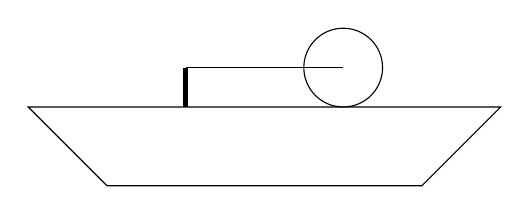
\begin{tikzpicture}
		\def\l{4};
		\def\h{1};
		\def\R{0.5};
		\def\angle{30};
	
		\draw ({-\l/2},0) -- ({\l/2},0) -- ++({\l/4},{\l/4}) -- ++(-{3*\l/2},0) -- cycle;
		\draw [ultra thick] ({-\l/4},{\l/4}) -- ++(0,{\R});
		\draw ({-\l/4},{\l/4 + \R}) -- ({\l/4},{\l/4 + \R});
		\draw ({\l/4},{\l/4 + \R}) circle [radius = \R];
	\end{tikzpicture}
\end{example}

\begin{solution}
	Let the mass of the cylinder and the mass of the boat be $m_1$ and $m_2$ respectively.\\
	Let the velocity of the cylinder and the velocity of the boat be $m_1$ and $m_2$ respectively.
	By COLM,
	\begin{align*}
		m_1 v_1 + m_2 v_2 &= 0\\
		\therefore m_1 v_1 &= - m_2 v_2\\
		\therefore m_1 v_1 &= - m_2 (v_1 + \omega R)
	\end{align*}
	\begin{align*}
		m_1 a_1 + m_2 a_2 &= 0\\
		\therefore m_1 a_1 + m_2 a_1 + m_2 \alpha R &= 0\\
		\therefore (m_1 + m_2) a_1 + m_2 \alpha R &= 0\\
		\therefore (m_1 + m_2) a_1 + m_2 \dfrac{F R}{\dfrac{3}{2} m_2 R^2} R &= 0\\
		\therefore (m_1 + m_2) a_1 + \dfrac{2}{3} F &= 0\\
		\therefore a_1 &= -\dfrac{2F}{3m_1 + m_2}\\
		\therefore a_2 &= \dfrac{m_1}{m_2} \cdot \dfrac{2F}{3m_1 + m_2}
	\end{align*}
	\begin{align*}
		v_1 &= a T\\
		&= \dfrac{2F}{3m_1 + m_2} T
	\end{align*}
	After $t = T$, the velocity does not change.
\end{solution}

\begin{example}
	A cylinder of mass $m$ and radius $R$ is attached to an axis with a spring of coefficient $k$. The cylinder is constrained to move in a straight line. The axis is rotating with $\Omega$. Find $\omega_0$, the angular frequency of the oscillations.
\end{example}

\begin{solution}
	Let the natural length of the spring be $L$.\\
	As viewed from inside the system, at equilibrium,
	\begin{align*}
		k x_0 &= m \Omega^2 (L + x_0)
	\end{align*}
	When the spring is extended by $x$,
	\begin{align*}
		m \ddot{x} &= - k(x_0 + x) + m \Omega^2 (L + x_0 + x) + f\\
		\therefore m \ddot{x} &= m \Omega^2 x + f - k x\\
		&= - (k - m \Omega^2) x + f
	\end{align*}
	As the cylinder is rolling without slipping
	\begin{align*}
		f R &= \dfrac{1}{2} m R^2 \alpha\\
		&= -\dfrac{1}{2} m R \ddot{x}\\
		\therefore f &= -\dfrac{1}{2} m \ddot{x}
	\end{align*}
	Therefore,
	\begin{align*}
		m \ddot{x} &= - (k - m \Omega^2) x - \dfrac{1}{2} m \ddot{x}\\
		\therefore \dfrac{3}{2} m \ddot{x} &= - (k - m \Omega^2) x\\
		\therefore \omega_0 &= \sqrt{\dfrac{2(k - m \Omega^2)}{3 m}}
	\end{align*}
\end{solution}

\begin{example}
	A pendulum is made of a rod of length $l$ and mass $m_1$ and a ball of mass $m_2$ and radius $R$. The ball's centre is at a distance $x$ from the axis. 
		\begin{enumerate}
			\item Find the position of the centre of mass with respect to the pivot point. 
			\item Find the moment of inertia of the pendulum with respect to the pivot axis. 
			\item Assuming small oscillations, find the frequency of oscillations. 
			\item The ball is released when the pendulum is vertical. The ball rotates with $\omega$. Assuming $x = L$ and the oscillations start at $\theta = \dfrac{\pi}{6}$, and $m_1 = m_2$, find $\omega$.
		\end{enumerate}
\end{example}

\begin{solution}
	\begin{align*}
		d_{\textnormal{COM}} &= \dfrac{m_1 \dfrac{L}{2} + m_2 x}{m_1 + m_2}\\
		&= \dfrac{m_1 L + 2 m_2 x}{2 (m_1 + m_2)}
	\end{align*}
	\begin{align*}
		I &= \dfrac{m_1 L^2}{3} + \dfrac{2}{5} m_2 R^2 + m_2 x^2
	\end{align*}
	\begin{align*}
		\omega_0 &= \sqrt{\dfrac{d_{\textnormal{COM}} (m_1 + m_2) g}{I}}
	\end{align*}
	~\\
	~\\
	By COME,
	\begin{align*}
		2 m g \cdot d \left( 1 - \dfrac{\sqrt{3}}{2} \right) &= \dfrac{1}{2} I \Omega^2
	\end{align*}
	\begin{align*}
		I &= \dfrac{m L^2}{3} + \dfrac{2}{5} m R^2 + m L^2\\
		&= m \left( \dfrac{4 L^2}{3} + \dfrac{2}{5} R^2 \right)
	\end{align*}
	Therefore,
	\begin{align*}
		\dfrac{4 m g d \left( 1 - \dfrac{\sqrt{3}}{2} \right)}{I} &= \Omega^2\\
		\therefore \sqrt{\dfrac{3 g L \left( 1 - \dfrac{\sqrt{3}}{2} \right)}{\left( \dfrac{4 L^2}{3} + \dfrac{2}{5} R^2 \right)}} &= \Omega
	\end{align*}
	The top of the ball has velocity $(L - R) \Omega$ and the bottom has velocity $(L + R) \Omega$. Therefore, the ball will rotate with $\Omega$ after it is released.
\end{solution}

\begin{example}
	Two rods of length $L$ each are moving with velocities $v$ towards each other. The top of the first rod is at a vertical distance $x L$ from the bottom of the second rod. After the rods collide, they stick together. Find the angular velocity of rotation of the entire body.\\
	\begin{tikzpicture}
		\def\L{4};
		\def\x{0.4};
		
		\draw ({\L/2}, {(\x/2)*\L}) -- ++(-90:\L);
		\draw ({-\L/2}, {-(\x/2)*\L}) -- ++(90:\L);
		
		\begin{scope}[dashed]
			\draw ({\L/2}, {(\x/2)*\L}) -- ++(180:\L);
			\draw ({-\L/2}, {(-\x/2)*\L}) -- ++(0:\L);
		\end{scope}
		
		\draw [|<->|, xshift = 20] ({\L/2}, {(\x/2)*\L}) -- ++(-90:{\x*\L}) node [midway, fill = white] {$xL$};
	\end{tikzpicture}
\end{example}

\begin{solution}
	By COAM about the centre of mass,
	\begin{align*}
		2 m v \left( \dfrac{L}{2} - \dfrac{xL}{2} \right) &= 2 \left( \dfrac{m L^2}{12} + m \left( \dfrac{L}{2} - \dfrac{xL}{2} \right)^2 \right) \omega\\
		\therefore \dfrac{v}{2} - \dfrac{x v}{2} &= \left( \dfrac{L}{12} + L \left( \dfrac{1}{2} - \dfrac{x}{2} \right)^2 \right) \omega\\
		\therefore \omega &= \dfrac{1 - x}{v \left( \dfrac{L}{6} + L (1 - x)^2 \right)}
	\end{align*}
\end{solution}

\end{document}